\def\panelAnnoBubbleMajorRadius{0.35cm}
\def\panelAnnoBubbleMinorRadius{0.25cm}
\def\panelAnnoHandleLength{6cm}
\def\panelAnnoBendLength{2cm}
\def\panelAnnoOpacity{0.0}

\subtikzpicturedef{subCoreBlockPanels} {
    origin%
} {
    \draw (#1-start) coordinate (#1-origin);

    \draw
    node (#1-img) [
        inner sep = 0pt,
        outer sep = 0pt,
    ] {
        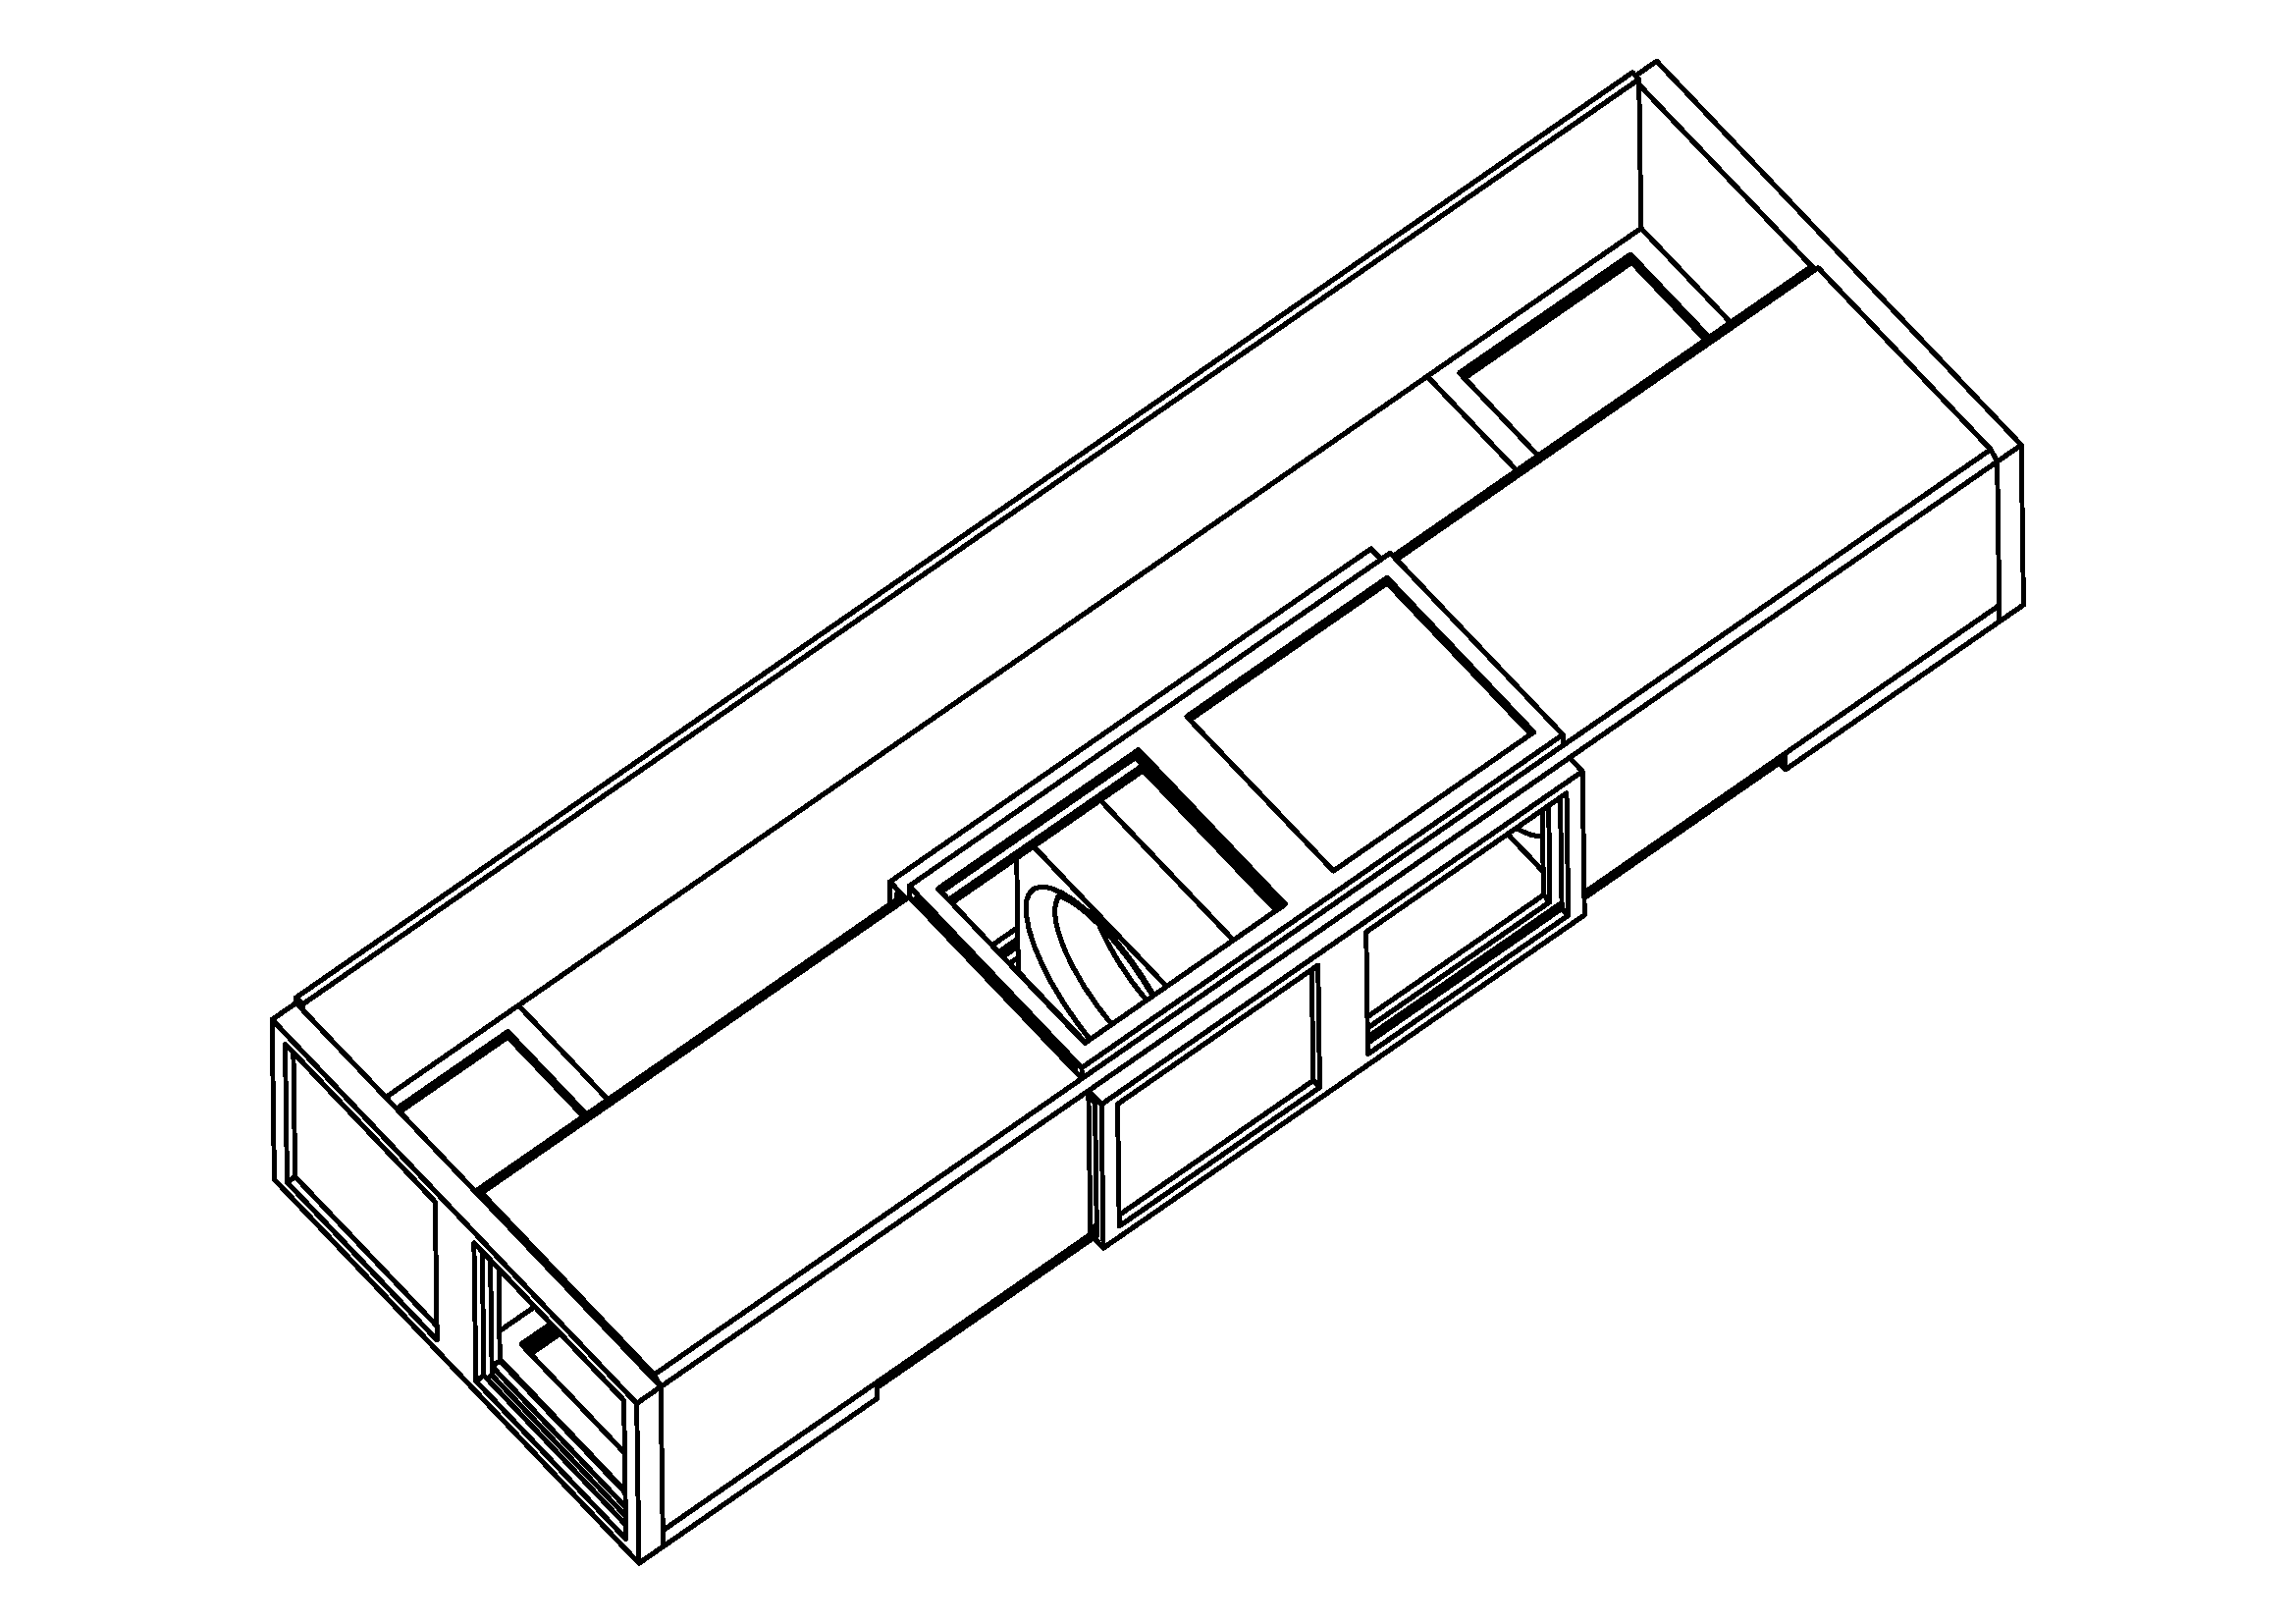
\includegraphics [
        ] {\subfix{pics/ortho_open.pdf}}
    }
    ;

    \draw
    (#1-img.north west) ++(81mm, -261mm) coordinate (#1-sidePanelOne)
    (#1-img.north west) ++(351mm, -58mm) coordinate (#1-sidePanelTwo)
    (#1-img.north west) ++(142mm, -267mm) coordinate (#1-botPanelOne)
    (#1-img.north west) ++(340mm, -130mm) coordinate (#1-botPanelTwo)
    % (#1-img.north west) ++(219mm, -147mm) coordinate (#1-midPanelCenter)
    (#1-img.north west) ++(223mm, -158mm) coordinate (#1-midPanelCenter)
    ;

    \draw
    (#1-sidePanelTwo) ++(\panelAnnoHandleLength, 0) coordinate (#1-sidePanelTwoMid)
    (#1-sidePanelTwoMid) ++(-45:\panelAnnoBendLength) coordinate (#1-sidePanelTwoEnd)

    (#1-sidePanelOne) ++(-{(\panelAnnoHandleLength * 1.5)}, 0) coordinate (#1-sidePanelOneMid)
    (#1-sidePanelOneMid) ++(135:\panelAnnoBendLength) coordinate (#1-sidePanelOneEnd)

    (#1-botPanelOne) ++(-45:\panelAnnoBendLength) coordinate (#1-botPanelOneMid)
    (#1-botPanelOneMid) ++(\panelAnnoHandleLength, 0) coordinate (#1-botPanelOneEnd)

    (#1-botPanelTwo) ++(-45:\panelAnnoBendLength) coordinate (#1-botPanelTwoMid)
    (#1-botPanelTwoMid) ++(\panelAnnoHandleLength, 0) coordinate (#1-botPanelTwoEnd)
    ;

    \draw [
        font = \HUGE,
    ]
    (#1-sidePanelOneEnd)
    node (#1-sidePanelOneNode) [
        left = 0.7cm,
    ] {
        \texttt{SIDE PANEL 01}
    }
    ;

    \draw [
        font = \HUGE,
    ]

    %% side panel 01 label

    (#1-sidePanelTwoEnd)
    node (#1-sidePanelTwoNode) [
        right = 0.7cm,
    ] {
        \texttt{SIDE PANEL 02}
    }

    %% bottom panel 02 label

    (#1-botPanelTwoEnd -| #1-sidePanelTwoNode.east)
    node (#1-botPanelTwoNode) [
        anchor = east,
    ] {
        \texttt{BOTTOM PANEL 02}
    }

    %% bottom panel 01 label

    (#1-botPanelOneEnd -| #1-botPanelTwoNode.east)
    node (#1-botPanelOneNode) [
        anchor = east,
    ] {
        \texttt{BOTTOM PANEL 01}
    }

    ;

    %% middle panels

    \draw [
        dash pattern = {on 0.5cm off 0.25cm},
        colorShadowGray,
        line width = 3pt,
    ]
    (#1-midPanelCenter) circle (6cm)
    ;

    \fill [
        fill = colorShadowGray,
        opacity = \panelAnnoOpacity,
    ]
    (#1-midPanelCenter) circle (5.5cm)
    ;

    \draw [
        rounded corners = 0.25cm,
        line width = 2pt,
    ]
    (#1-midPanelCenter) ++(-45:6cm) coordinate (#1-midPanelCenterStart)
    ++(-45:\panelAnnoBendLength) coordinate (#1-midPanelCenterMid)
    ++(\panelAnnoHandleLength, 0) coordinate (#1-midPanelCenterEnd)
    ;

    \draw
    (#1-midPanelCenterEnd -| #1-botPanelTwoNode.east)
    node (#1-tmpNode1) [
        anchor = east,
        font = \HUGE,
    ] {
        \texttt{MIDDLE PANEL 01}
    }
    (#1-tmpNode1.south)
    node (#1-tmpNode) [
        below = 0.7cm,
        font = \HUGE,
    ] {
        \texttt{MIDDLE PANEL 02}
    }
    (#1-tmpNode.south)
    node (#1-tmpNode) [
        below = 0.7cm,
        font = \HUGE,
    ] {
        \texttt{MIDDLE PANEL 03}
    }
    ;


    \draw [
        rounded corners = 0.25cm,
        line width = 2pt,
    ]
    (#1-tmpNode1.west) ++(-0.7cm, 0) coordinate (#1-midPanelCenterEnd)
    (#1-midPanelCenterStart) -- (#1-midPanelCenterMid) -- (#1-midPanelCenterEnd)
    ;

    \draw [
        fill = bgcol,
        line width = 2pt,
    ]
    (#1-midPanelCenterEnd) circle (\panelAnnoBubbleMinorRadius)
    ;

    %% circles

    \draw
    (#1-botPanelOneEnd -| #1-botPanelOneNode.west) ++(-0.7cm, 0) coordinate (#1-botPanelOneEnd)
    (#1-botPanelTwoEnd -| #1-botPanelTwoNode.west) ++(-0.7cm, 0) coordinate (#1-botPanelTwoEnd)
    (#1-sidePanelTwoEnd -| #1-sidePanelTwoNode.west) ++(-0.7cm, 0) coordinate (#1-sidePanelTwoEnd)
    ;

    \foreach \x/\y/\z in {
        sidePanelOne/sidePanelOneMid/sidePanelOneEnd,
        sidePanelTwo/sidePanelTwoMid/sidePanelTwoEnd,
        botPanelOne/botPanelOneMid/botPanelOneEnd,
        botPanelTwo/botPanelTwoMid/botPanelTwoEnd%
    } {
        \draw [
            line width = 2pt,
            rounded corners = 0.25cm,
            % ultra thick,
        ]
        (#1-\x) -- (#1-\y) -- (#1-\z)
        ;
    }


    \foreach \x in {
        sidePanelOne,
        sidePanelTwo,
        botPanelOne,
        botPanelTwo%
    } {
        \draw [
            fill = bgcol,
            line width = 2pt,
        ]
        (#1-\x) circle (\panelAnnoBubbleMajorRadius)
        ;
    }

    \foreach \x in {
        sidePanelOneEnd,
        sidePanelTwoEnd,
        botPanelOneEnd,
        botPanelTwoEnd%
    } {
        \draw [
            fill = bgcol,
            line width = 2pt,
        ]
        (#1-\x) circle (\panelAnnoBubbleMinorRadius)
        ;
    }

    %% chambers

    \draw
    (#1-img.north west) ++(135mm, -211mm) coordinate (#1-heaterChamber)
    (#1-img.north west) ++(302mm, -95mm) coordinate (#1-coolerChamber)
    (#1-img.north west) ++(120mm, -148mm) coordinate (#1-commonChamber)
    ;

    \draw [
        dash pattern = {on 0.5cm off 0.25cm},
        colorShadowGray,
        line width = 3pt,
    ]
    (#1-heaterChamber) circle (2.5cm)
    (#1-coolerChamber) circle (2.5cm)
    (#1-commonChamber) circle (2.5cm)
    ;

    \draw [
    ]
    (#1-heaterChamber) ++(135:2.5cm) coordinate (#1-heaterChamberStart)
    (#1-heaterChamberStart) ++(135:\panelAnnoBendLength) coordinate (#1-heaterChamberMid)
    (#1-heaterChamberMid -| #1-sidePanelOneNode.west) coordinate (#1-heaterChamberNode)

    (#1-coolerChamber) ++(135:2.5cm) coordinate (#1-coolerChamberStart)
    (#1-coolerChamberStart) ++(135:{\panelAnnoBendLength * 3.5}) coordinate (#1-coolerChamberMid)
    (#1-coolerChamberMid -| #1-sidePanelOneNode.west) coordinate (#1-coolerChamberNode)

    (#1-commonChamber) ++(135:2.5cm) coordinate (#1-commonChamberStart)
    (#1-commonChamberStart) ++(135:\panelAnnoBendLength) coordinate (#1-commonChamberMid)
    (#1-commonChamberMid -| #1-sidePanelOneNode.west) coordinate (#1-commonChamberNode)
    ;

    \foreach \cord/\name in {
        coolerChamberNode/COOLING CHAMBER,
        heaterChamberNode/HEATING CHAMBER,
        commonChamberNode/COMMON CHAMBER%
    } {
        \draw [
            font = \HUGE,
        ]
        (#1-\cord)
        node (#1-\cord) [
            anchor = west,
        ] {
            \texttt{\name}
        }
        ;
    }

    \draw [
        rounded corners = 0.25cm,
        line width = 2pt,
    ]

    (#1-coolerChamberNode.east) ++(0.7cm, 0) coordinate (#1-coolerChamberEnd)
    (#1-coolerChamberStart) -- (#1-coolerChamberMid) -- (#1-coolerChamberEnd)

    (#1-heaterChamberNode.east) ++(0.7cm, 0) coordinate (#1-heaterChamberEnd)
    (#1-heaterChamberStart) -- (#1-heaterChamberMid) -- (#1-heaterChamberEnd)

    (#1-commonChamberNode.east) ++(0.7cm, 0) coordinate (#1-commonChamberEnd)
    (#1-commonChamberStart) -- (#1-commonChamberMid) -- (#1-commonChamberEnd)

    ;

    \foreach \x/\c in {
        coolerChamber/colorAlertNote,
        heaterChamber/colorAlertCaution,
        commonChamber/colorAlertTip%
    } {
        \fill [
            fill = \c,
        opacity = \panelAnnoOpacity,
        ]
        (#1-\x) circle (2.0cm)
        ;
    }

    \draw [
        fill = bgcol,
        line width = 2pt,
    ]
    (#1-coolerChamberEnd) circle (\panelAnnoBubbleMinorRadius)
    (#1-heaterChamberEnd) circle (\panelAnnoBubbleMinorRadius)
    (#1-commonChamberEnd) circle (\panelAnnoBubbleMinorRadius)
    ;

    \draw

    (#1-sidePanelTwoNode.east |- #1-img.north)
    node (#1-view) [
        anchor = south east,
        font = \HUGE,
    ] {
        \texttt{VIEW: BACK TOP RIGHT}
    }

    ;

}

\subtikzpictureactivate{subCoreBlockPanels}
